\label{appendix_c}

Some figures were produced for the project which have been included below for completeness. 


\begin{figure}[htbp]
    \centering
     
     \begin{subfigure}{0.4\textwidth}
         
         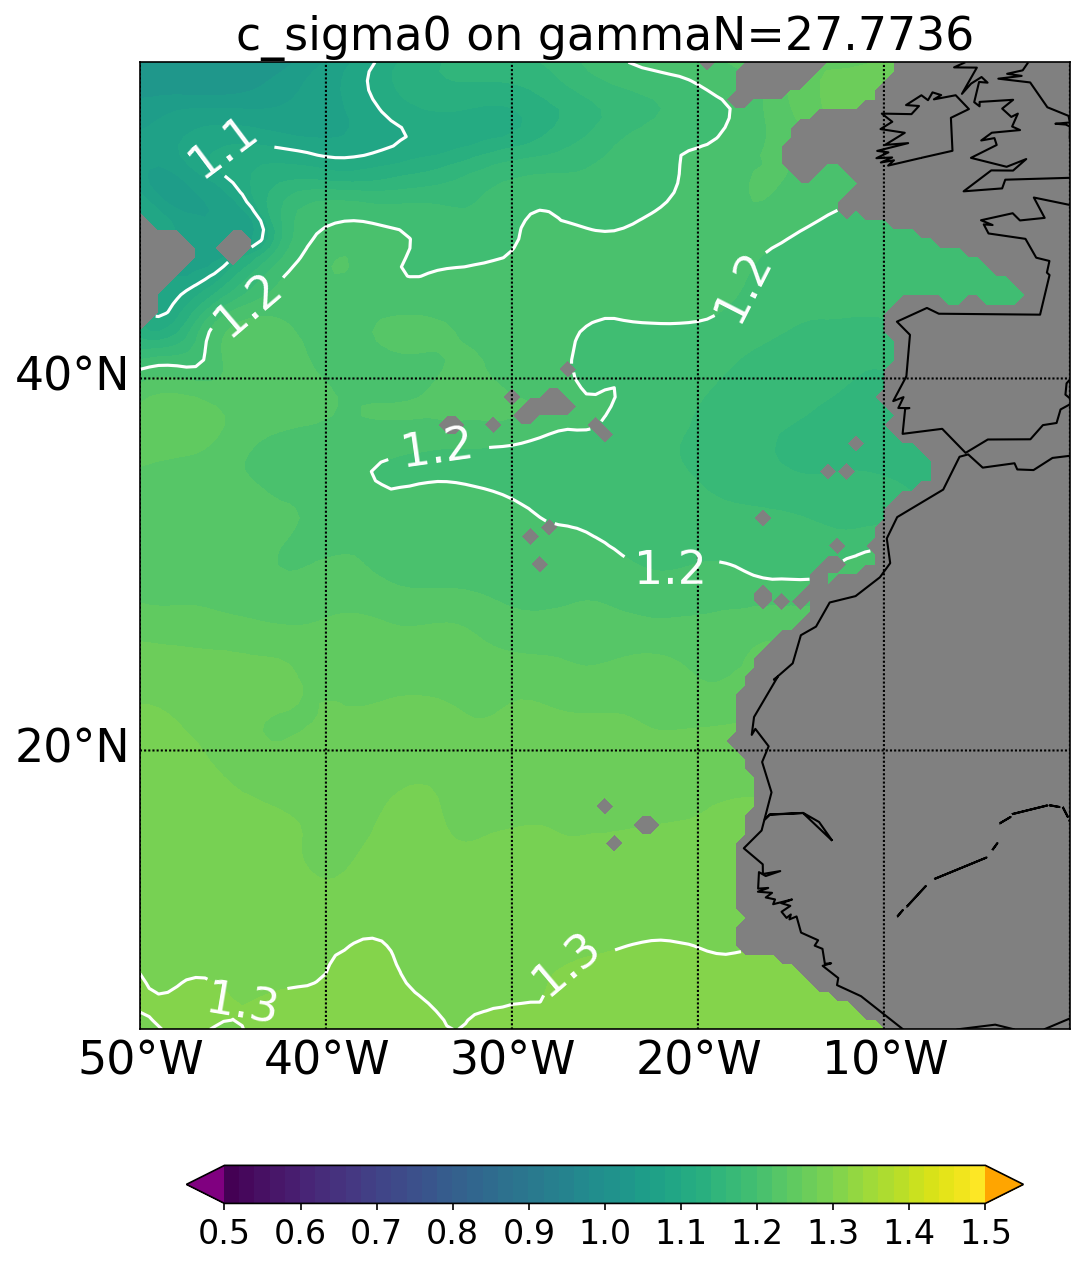
\includegraphics[width=\textwidth]{c/gibraltar_c/Map2dcyl_c_sigma0_on_gammaN_2777e-2_reg310Eto360E05Nto57N_1990to1998av_WOCE}
         \label{fig:subplot_gibraltar_c_sig0}
     \end{subfigure}
     \begin{subfigure}{0.4\textwidth}
         
         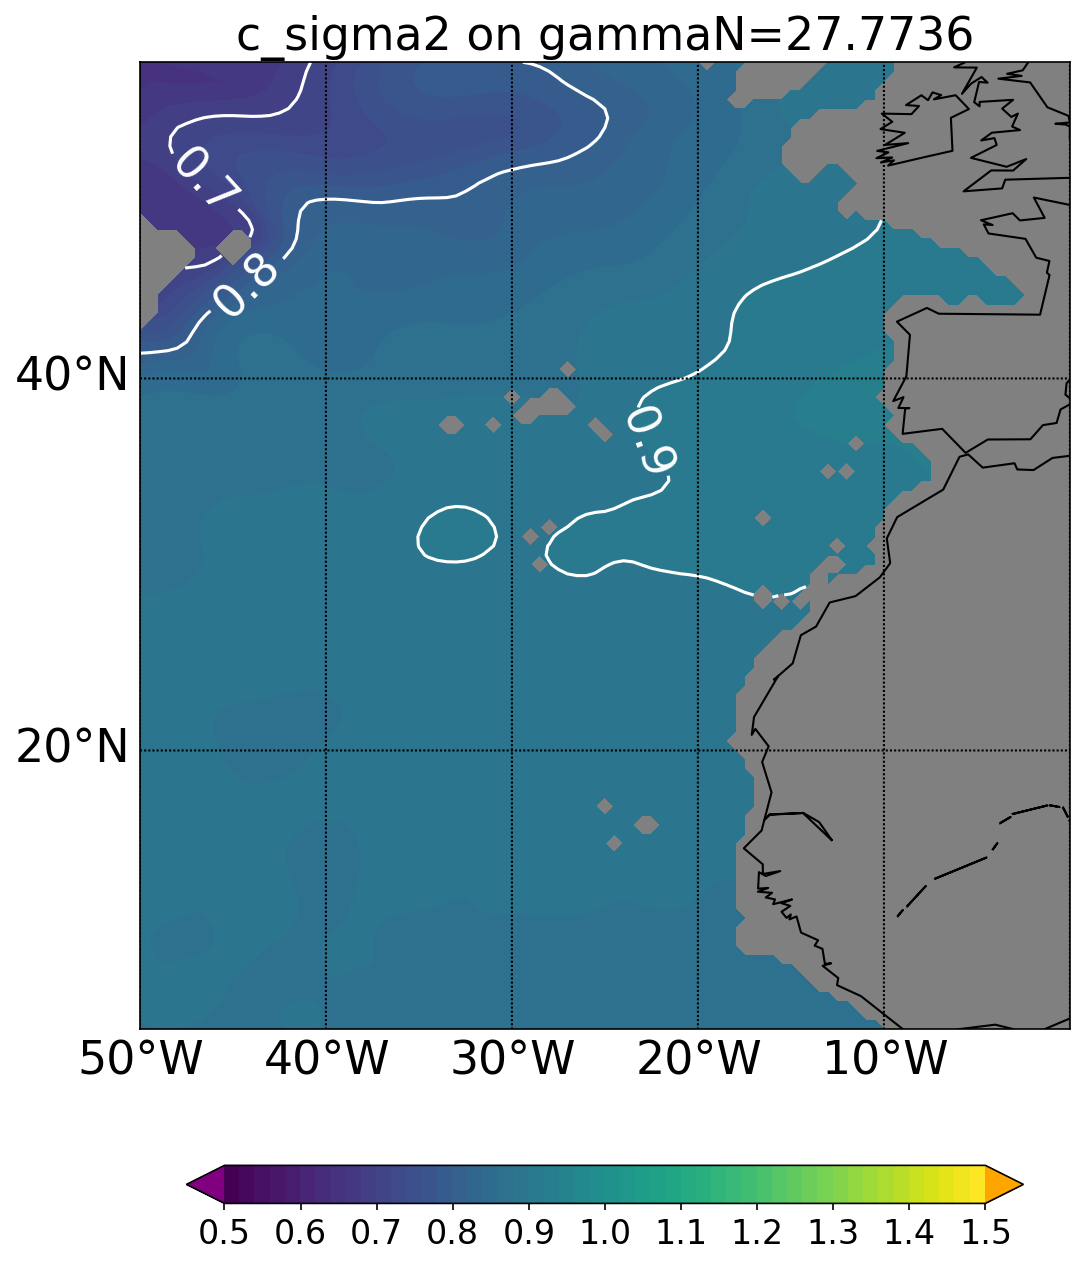
\includegraphics[width=\textwidth]{c/gibraltar_c/Map2dcyl_c_sigma2_on_gammaN_2777e-2_reg310Eto360E05Nto57N_1990to1998av_WOCE}
         \caption{Referenced to $p_{ref} = 2000$dbar}
         \label{fig:subplot_gibraltar_c_sig2}
     \end{subfigure}
     
     \begin{subfigure}{0.4\textwidth}
         
         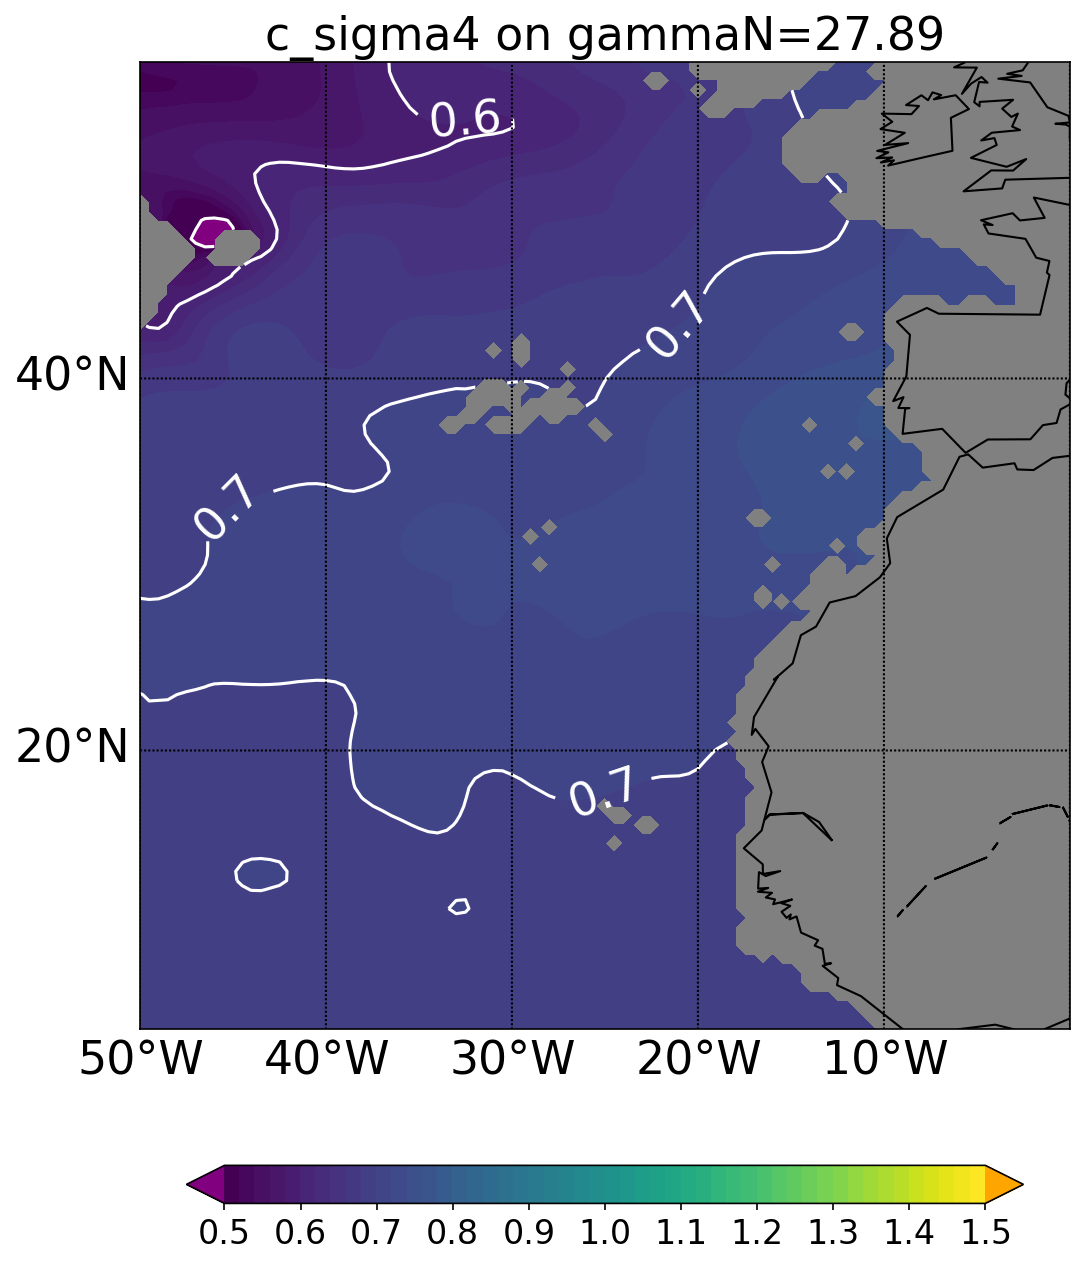
\includegraphics[width=\textwidth]{c/atlantic_c/Map2dcyl_c_sigma4_on_gammaN_2789e-2_reg310Eto360E05Nto57N_1990to1998av_WOCE}
         \caption{Referenced to $p_{ref} = 4000$dbar}
         \label{fig:subplot_gibraltar_c_sig4}
     \end{subfigure}
     
    \caption{The ratio of expansion coefficients, $c$ for three reference pressures, 0, 2000 and 4000dbar which correspond to the $\sigma_0$, $\sigma_2$ and $\sigma_4$ potential density surfaces respectively, projected onto the neutral surface $\gamma_n = 27.7736$, Gibraltar region (see section \ref{subsubsection:spreadmethodgibraltarstraight})}
    \label{fig:gibraltar_c}
    
\end{figure}

\begin{figure}[htbp]
    \centering
     \begin{subfigure}[b]{0.4\textwidth}
         
         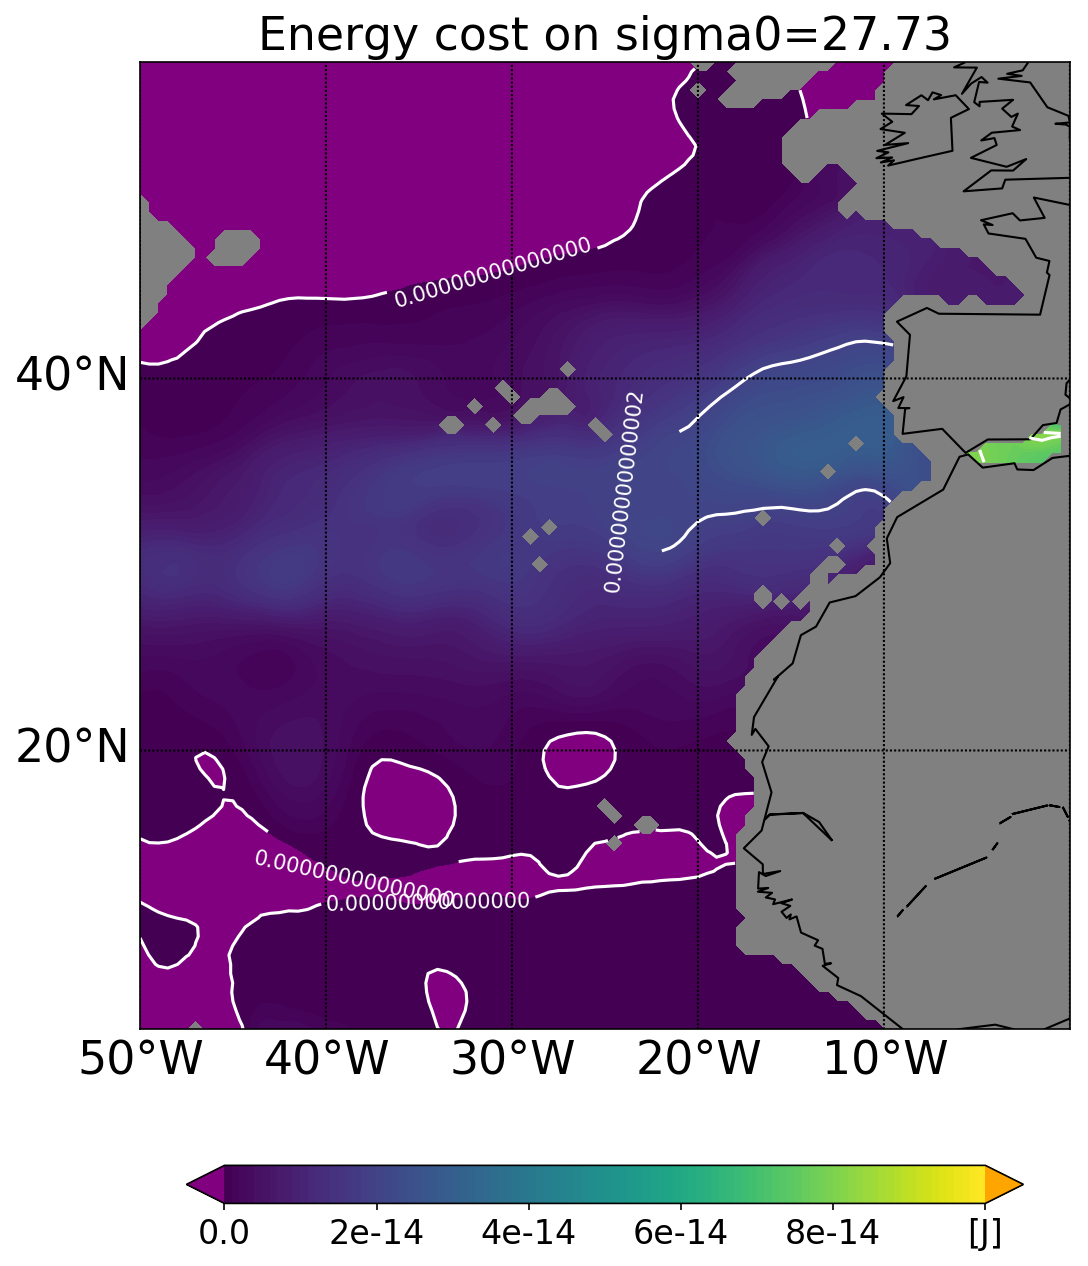
\includegraphics[width=\textwidth]{plots/energy/atlantic_energy/Map2dcyl_energy_on_sigma0_2773e-2_reg310Eto360E05Nto57N_1990to1998av_WOCE.png}
         \caption{$\frac{\Delta E}{d^2}$ on $\sigma_0 = 27.73$, Atlantic}
         \label{fig:subplot_atlantic_energy_sigma_0}
     \end{subfigure}
     \hfill
     \begin{subfigure}[b]{0.4\textwidth}
         
         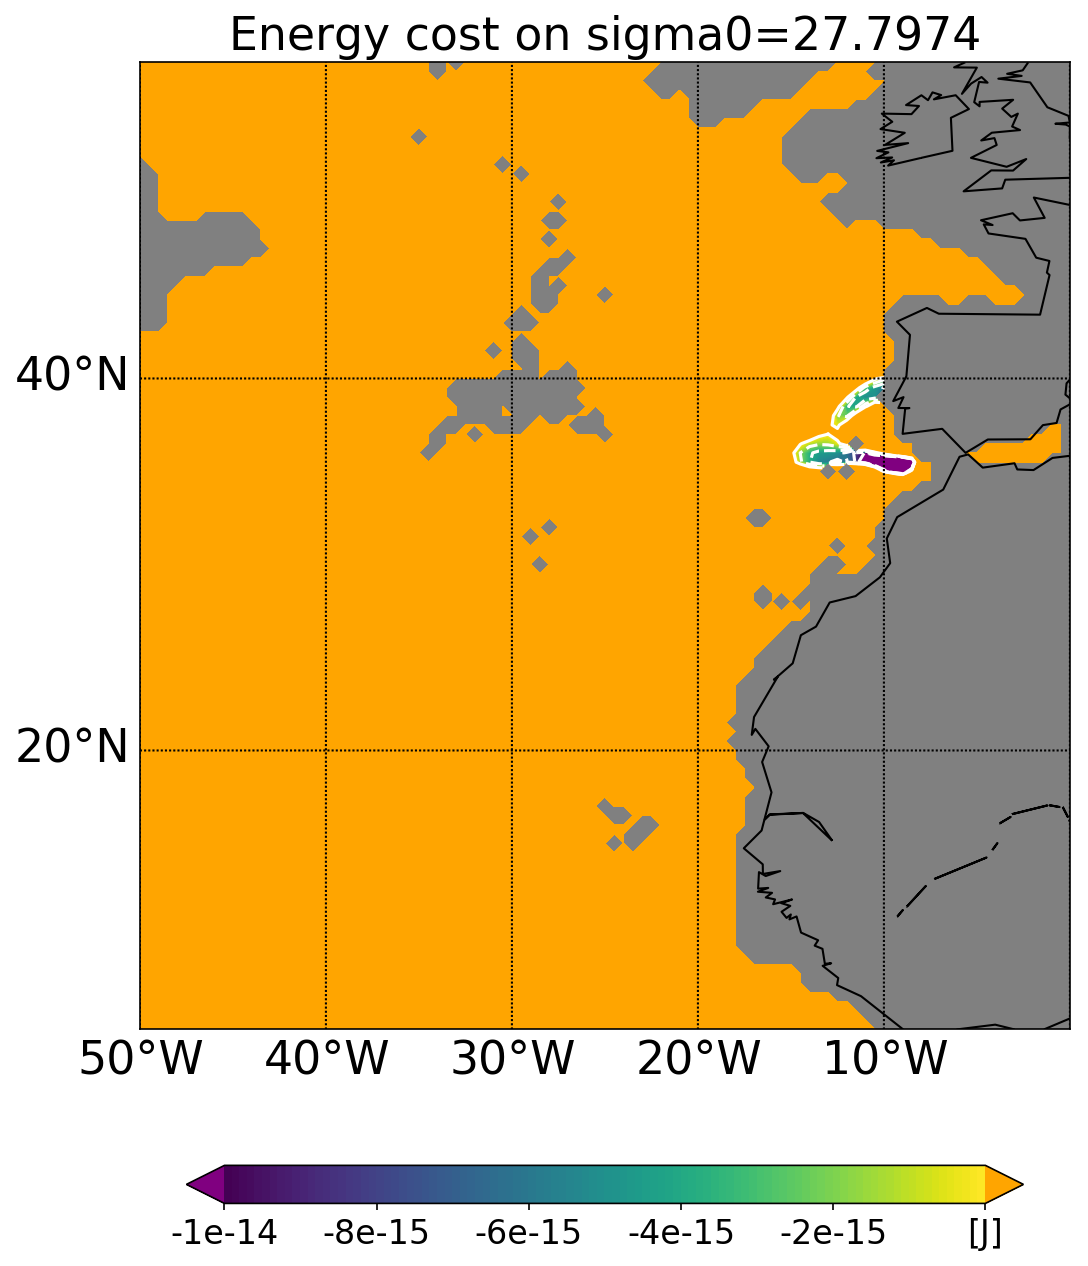
\includegraphics[width=\textwidth]{plots/energy/gibraltar_energy/Map2dcyl_neg_energy_on_sigma0_2779e-2_reg310Eto360E05Nto57N_1990to1998av_WOCE.png}
         \caption{$\frac{\Delta E}{d^2}$ on $\sigma_0 = 27.7974$, Gibraltar}
         \label{fig:subplot_gibraltar_energy_sigma_0}
     \end{subfigure}
     \hfill
      \begin{subfigure}[b]{0.4\textwidth}
         
         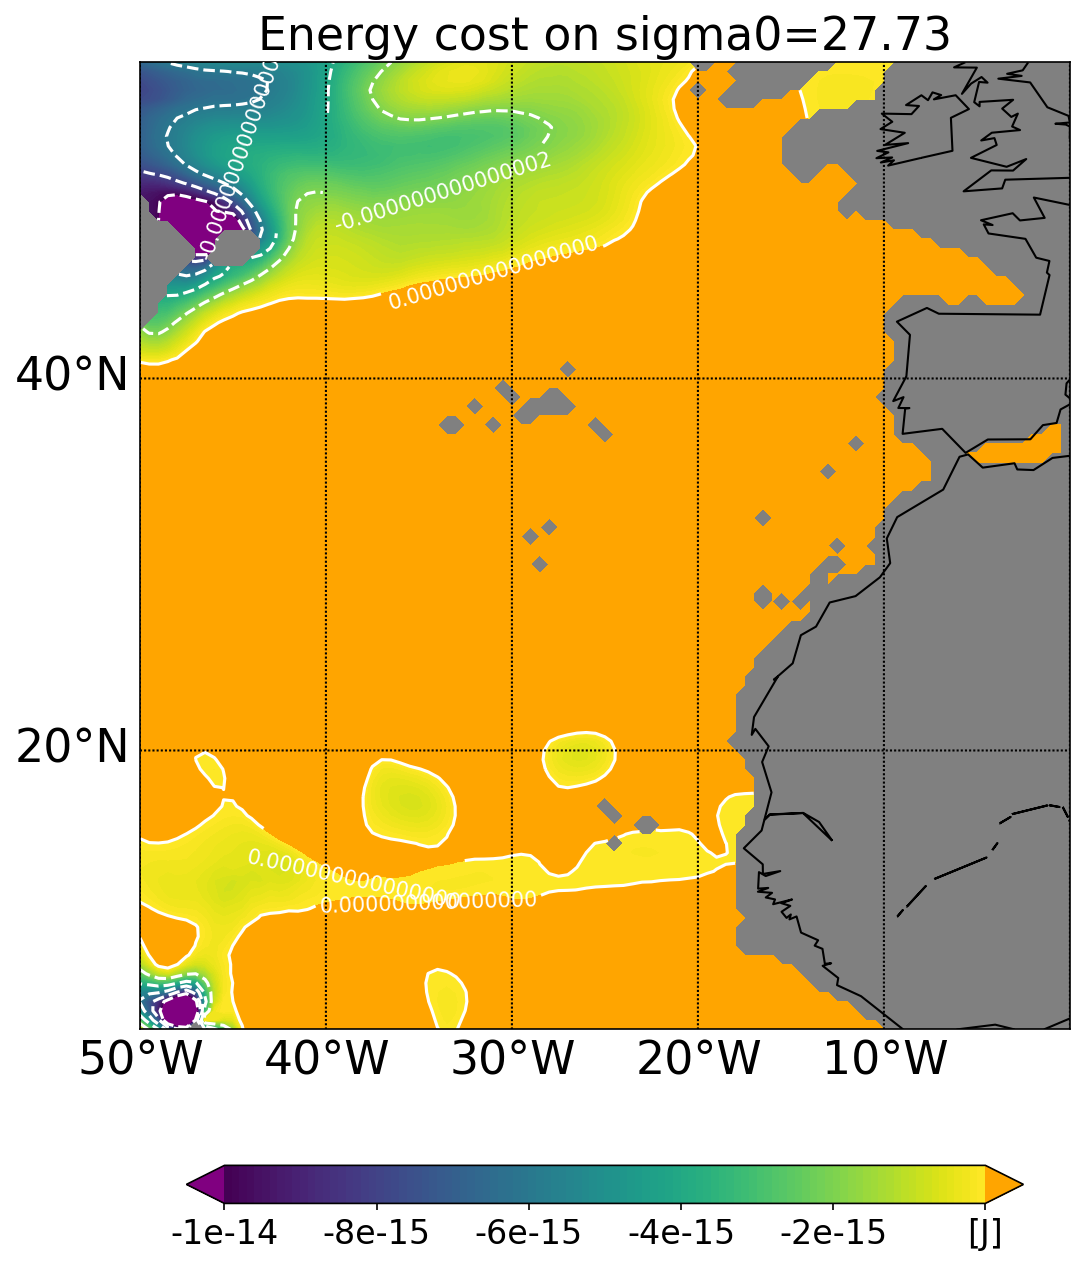
\includegraphics[width=\textwidth]{plots/energy/atlantic_energy/Map2dcyl_neg_energy_on_sigma0_2773e-2_reg310Eto360E05Nto57N_1990to1998av_WOCE.png}
         \caption{$\frac{\Delta E}{d^2}$ on $\sigma_0 = 27.73$, Atlantic}
         \label{fig:subplot_atlantic_neg_energy_sigma_0}
     \end{subfigure}
     \hfill
     \begin{subfigure}[b]{0.4\textwidth}
         
         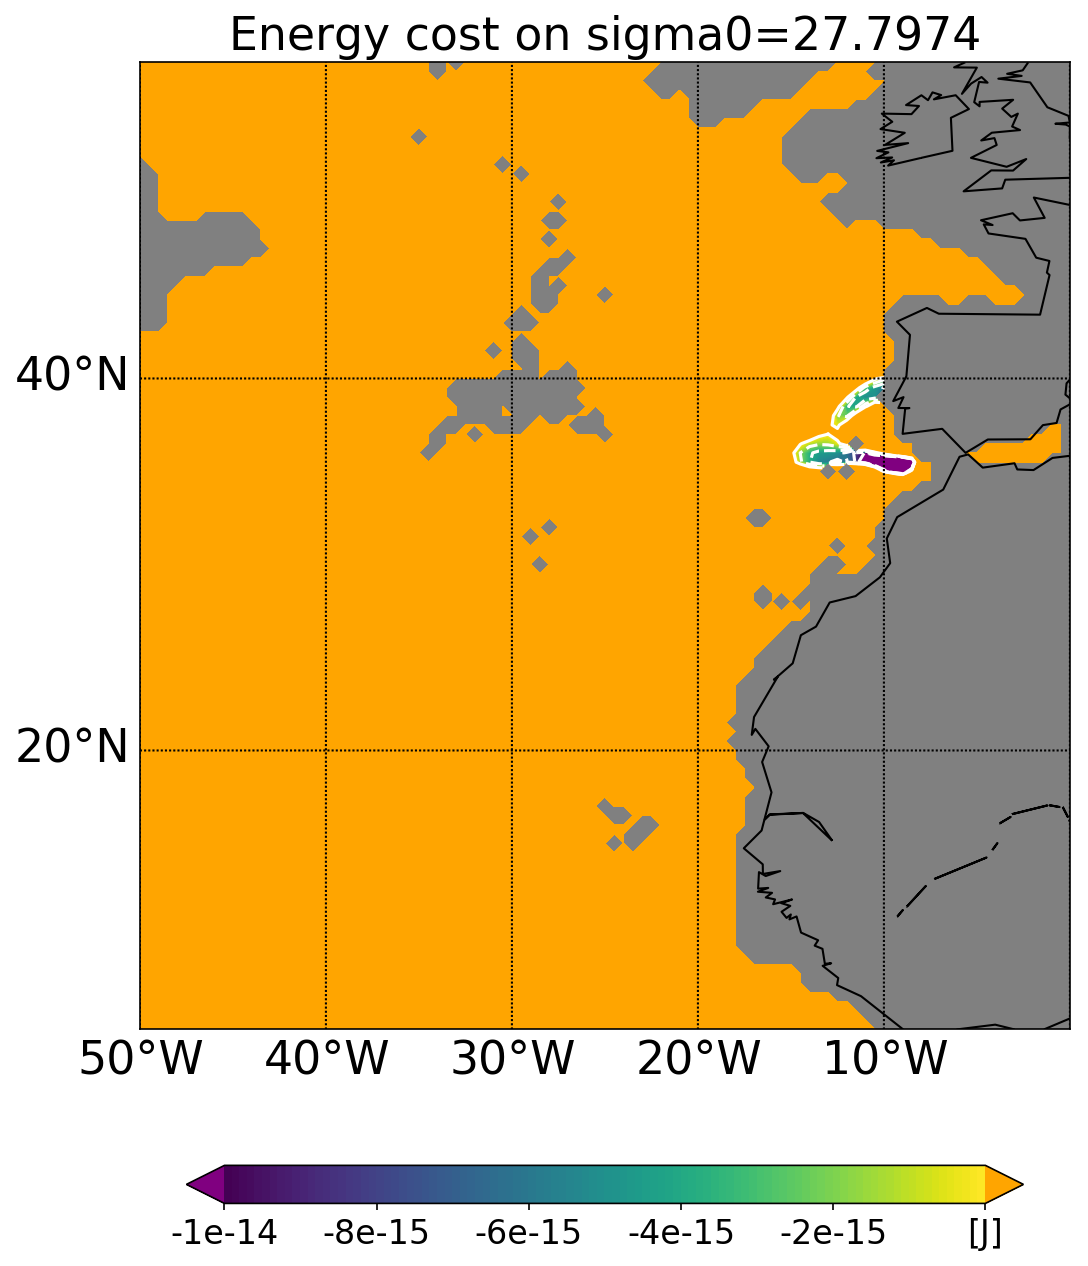
\includegraphics[width=\textwidth]{plots/energy/gibraltar_energy/Map2dcyl_neg_energy_on_sigma0_2779e-2_reg310Eto360E05Nto57N_1990to1998av_WOCE.png}
         \caption{$\frac{\Delta E}{d^2}$ on $\sigma_0 = 27.7974$, Gibraltar}
         \label{fig:subplot_gibraltar_neg_energy_sigma_0}
     \end{subfigure}
     
    \caption{The normalised energy cost, $\frac{\Delta E}{d^2}$, calculated on the the neutral surfaces $\sigma_0 = 27.73$ for the Atlantic region and  $\sigma_0 = 27.7974$ for the Gibraltar region (see section \ref{subsubsection:spreadmethodgibraltarstraight}). Figures (a) and (b) show positive energy cost, figures (c) and (d) show negative energy cost}
    \label{fig:energy_sigma_0}
    
\end{figure}

\begin{figure}[htbp]
    \centering
     \begin{subfigure}[b]{0.4\textwidth}
         
         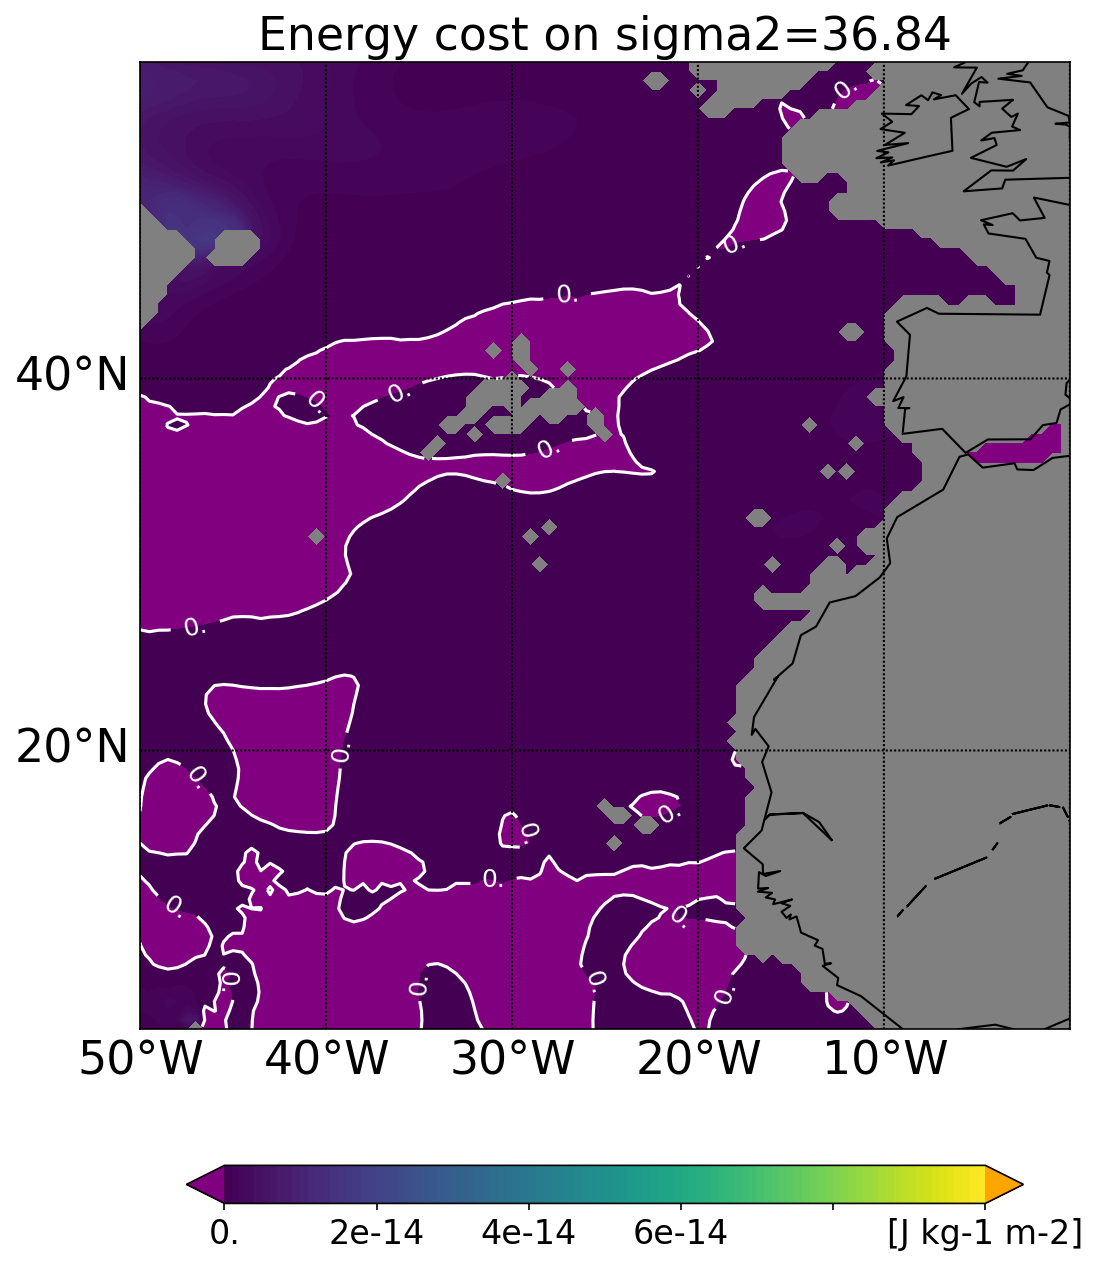
\includegraphics[width=\textwidth]{plots/energy/atlantic_energy/Map2dcyl_energy_on_sigma2_3684e-2_reg310Eto360E05Nto57N_1990to1998av_WOCE.png}
         \caption{$\frac{\Delta E}{d^2}$ on $\sigma_2 = 36.84$, Atlantic}
         \label{fig:subplot_atlantic_energy_sigma_2}
     \end{subfigure}
     \hfill
     \begin{subfigure}[b]{0.4\textwidth}
         
         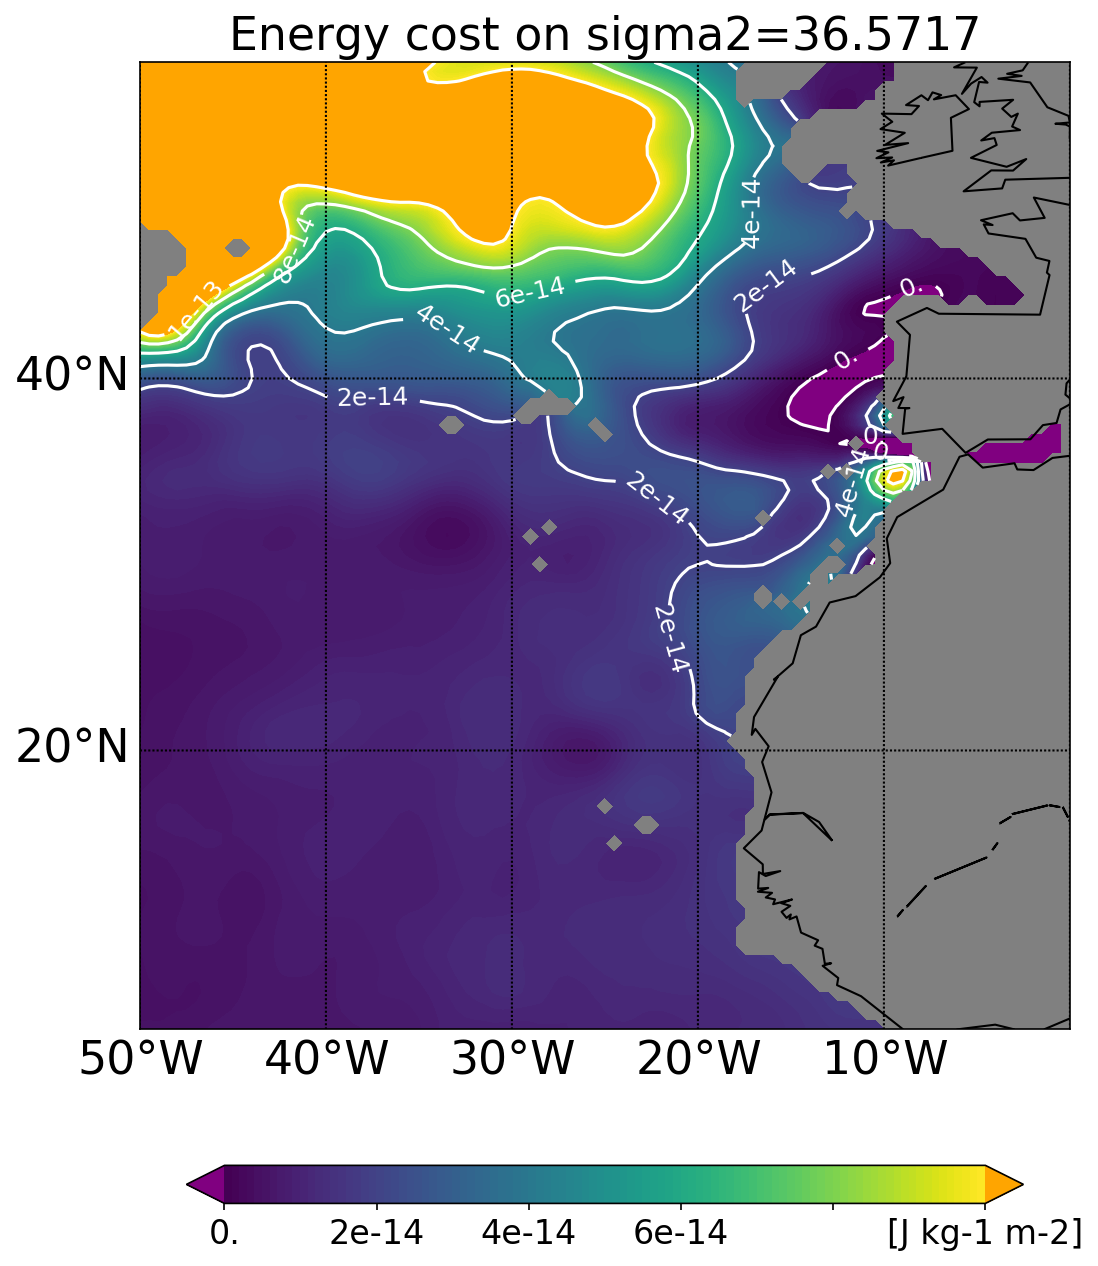
\includegraphics[width=\textwidth]{plots/energy/gibraltar_energy/Map2dcyl_energy_on_sigma2_3657e-2_reg310Eto360E05Nto57N_1990to1998av_WOCE.png}
         \caption{$\frac{\Delta E}{d^2}$ on $\sigma_2 = 36.5717$, Gibraltar}
         \label{fig:subplot_gibraltar_energy_sigma_2}
     \end{subfigure}
     \hfill
      \begin{subfigure}[b]{0.4\textwidth}
         
         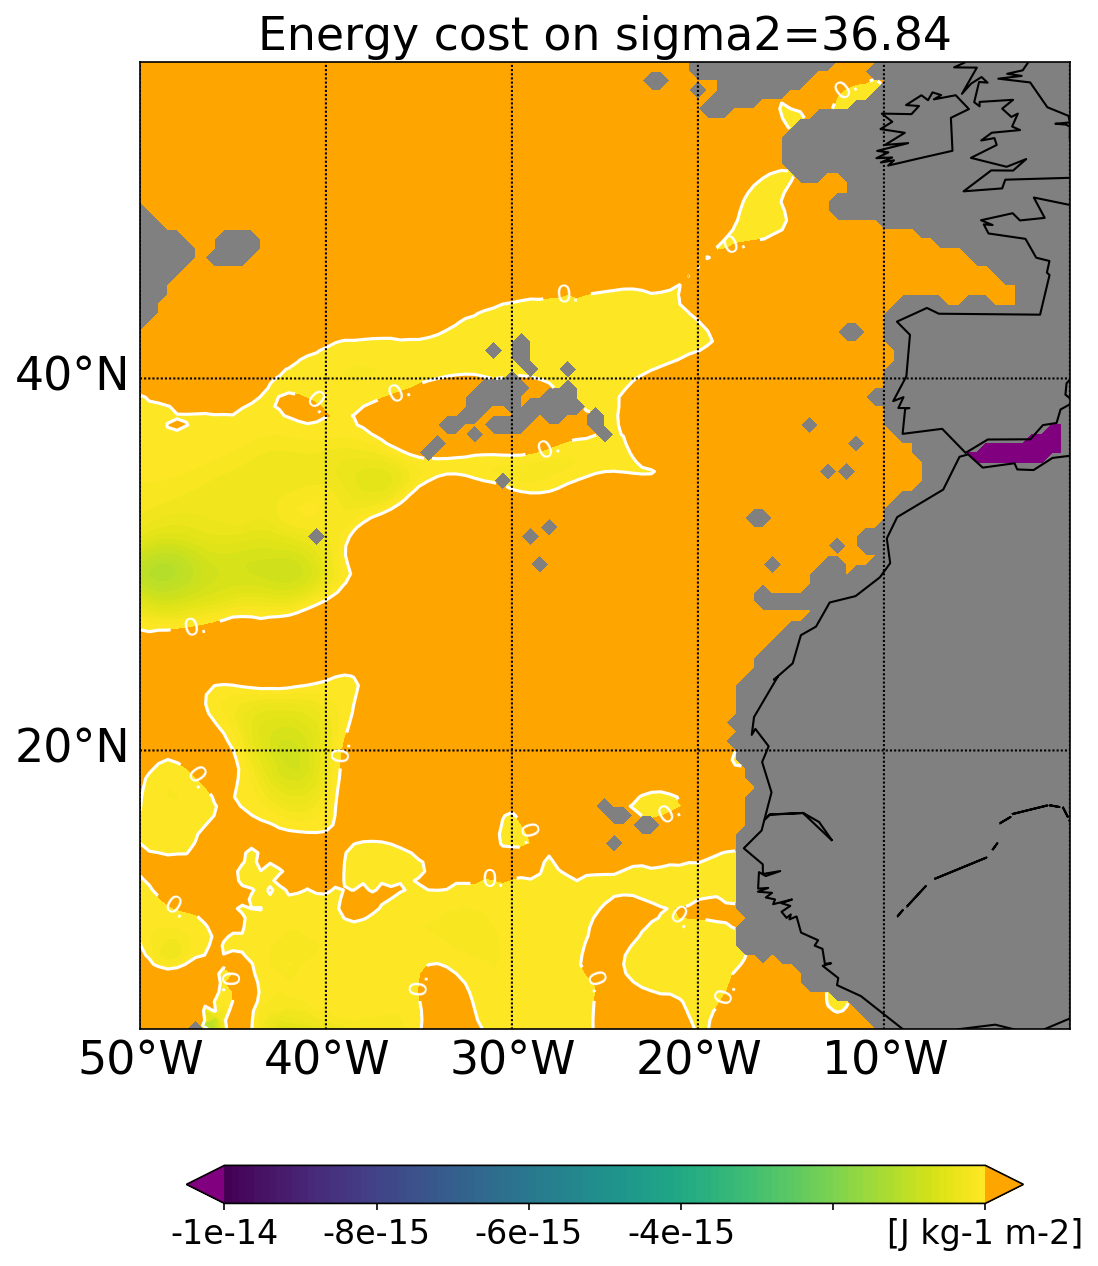
\includegraphics[width=\textwidth]{plots/energy/atlantic_energy/Map2dcyl_neg_energy_on_sigma2_3684e-2_reg310Eto360E05Nto57N_1990to1998av_WOCE.png}
         \caption{$\frac{\Delta E}{d^2}$ on $\sigma_2 = 36.84$, Atlantic}
         \label{fig:subplot_atlantic_neg_energy_sigma_2}
     \end{subfigure}
     \hfill
     \begin{subfigure}[b]{0.4\textwidth}
         
         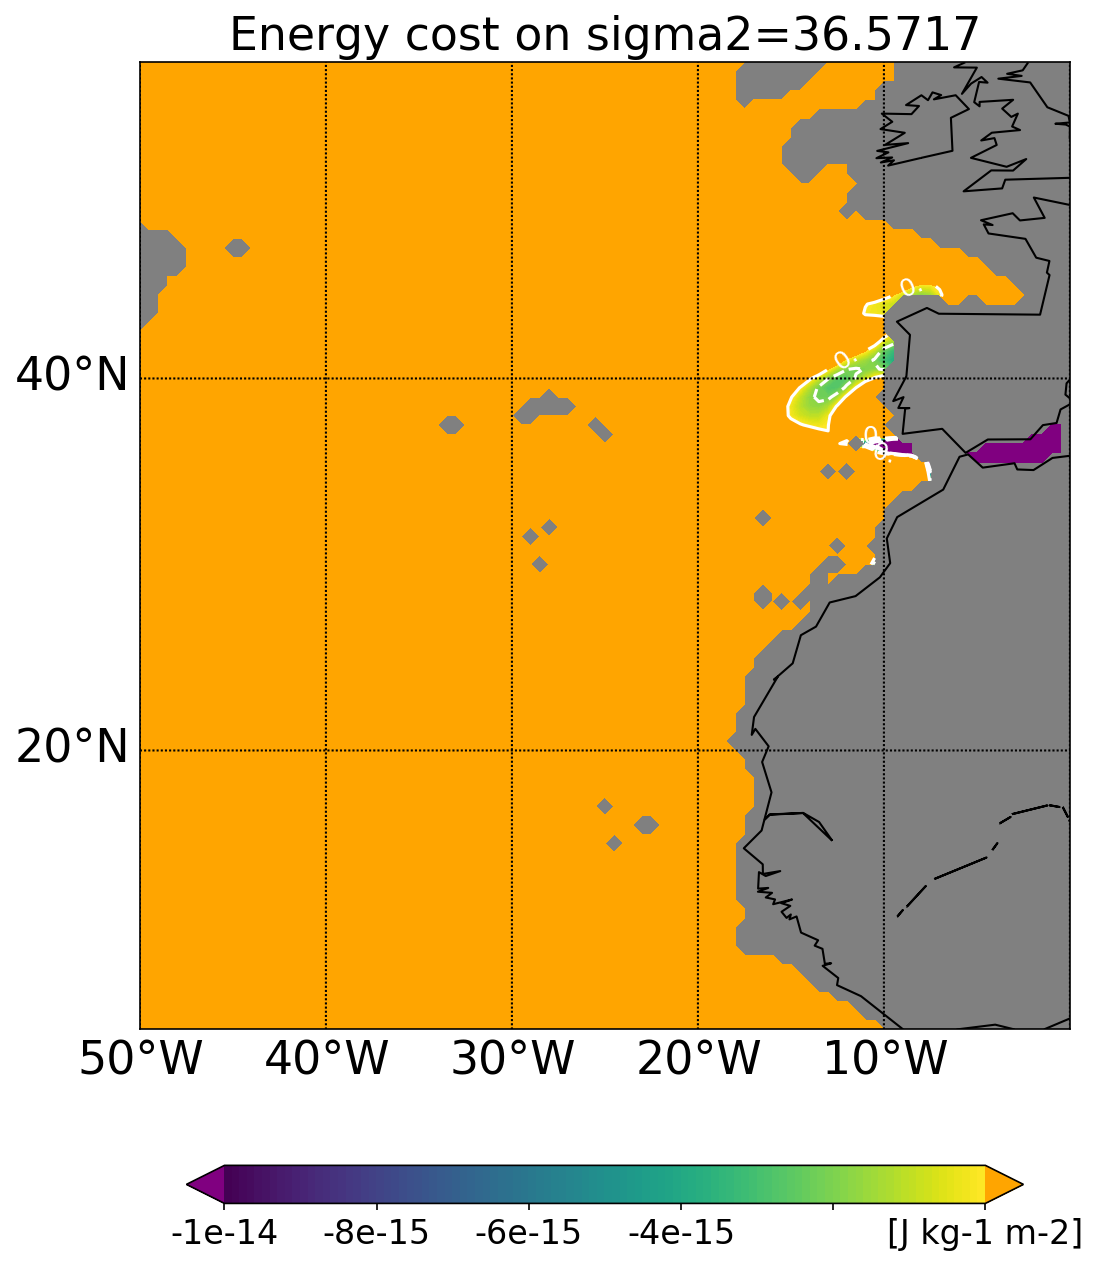
\includegraphics[width=\textwidth]{plots/energy/gibraltar_energy/Map2dcyl_neg_energy_on_sigma2_3657e-2_reg310Eto360E05Nto57N_1990to1998av_WOCE.png}
         \caption{$\frac{\Delta E}{d^2}$ on $\sigma_2 = 36.5717$, Gibraltar}
         \label{fig:subplot_gibraltar_neg_energy_sigma_2}
     \end{subfigure}
     
    \caption{The normalised energy cost, $\frac{\Delta E}{d^2}$, calculated on the the neutral surfaces $\sigma_2 = 36.84$ for the Atlantic region and  $\sigma_2 = 36.5717$ for the Gibraltar region (see section \ref{subsubsection:spreadmethodgibraltarstraight}). Figures (a) and (b) show positive energy cost, figures (c) and (d) show negative energy cost}
    \label{fig:energy_sigma_2}
    
\end{figure}
